\section{Результаты работы программы}

В данном разделе представлены результаты выполнения всех пунктов задания
лабораторной работы~1. Для каждого пункта приведён краткий обзор вывода
программного комплекса и соответствующая визуализация.

\subsection{Генерация графа по распределению Рэлея--Райса}

Генерируется связный ациклический неориентированный граф. Пользователь
вводит число вершин~$n$, параметры распределения~$a$ и~$h$. Число рёбер
и их распределение по степеням вершин определяются автоматически через
softmax-нормировку выборок из распределения Рэлея--Райса. Веса рёбер
также генерируются по тому же закону. На выходе программа выводит
матрицу смежности и список рёбер с весами.

Визуальное подтверждение корректности генерации весов представлено на рис.~\ref{fig:graph_gen}, где показана гистограмма сгенерированных значений с наложенной теоретической плотностью вероятности $f(z; a, h)$.

\begin{figure}[H]
    \centering
    
\includegraphics[width=0.7\linewidth]{images/lab1/graph.png}
    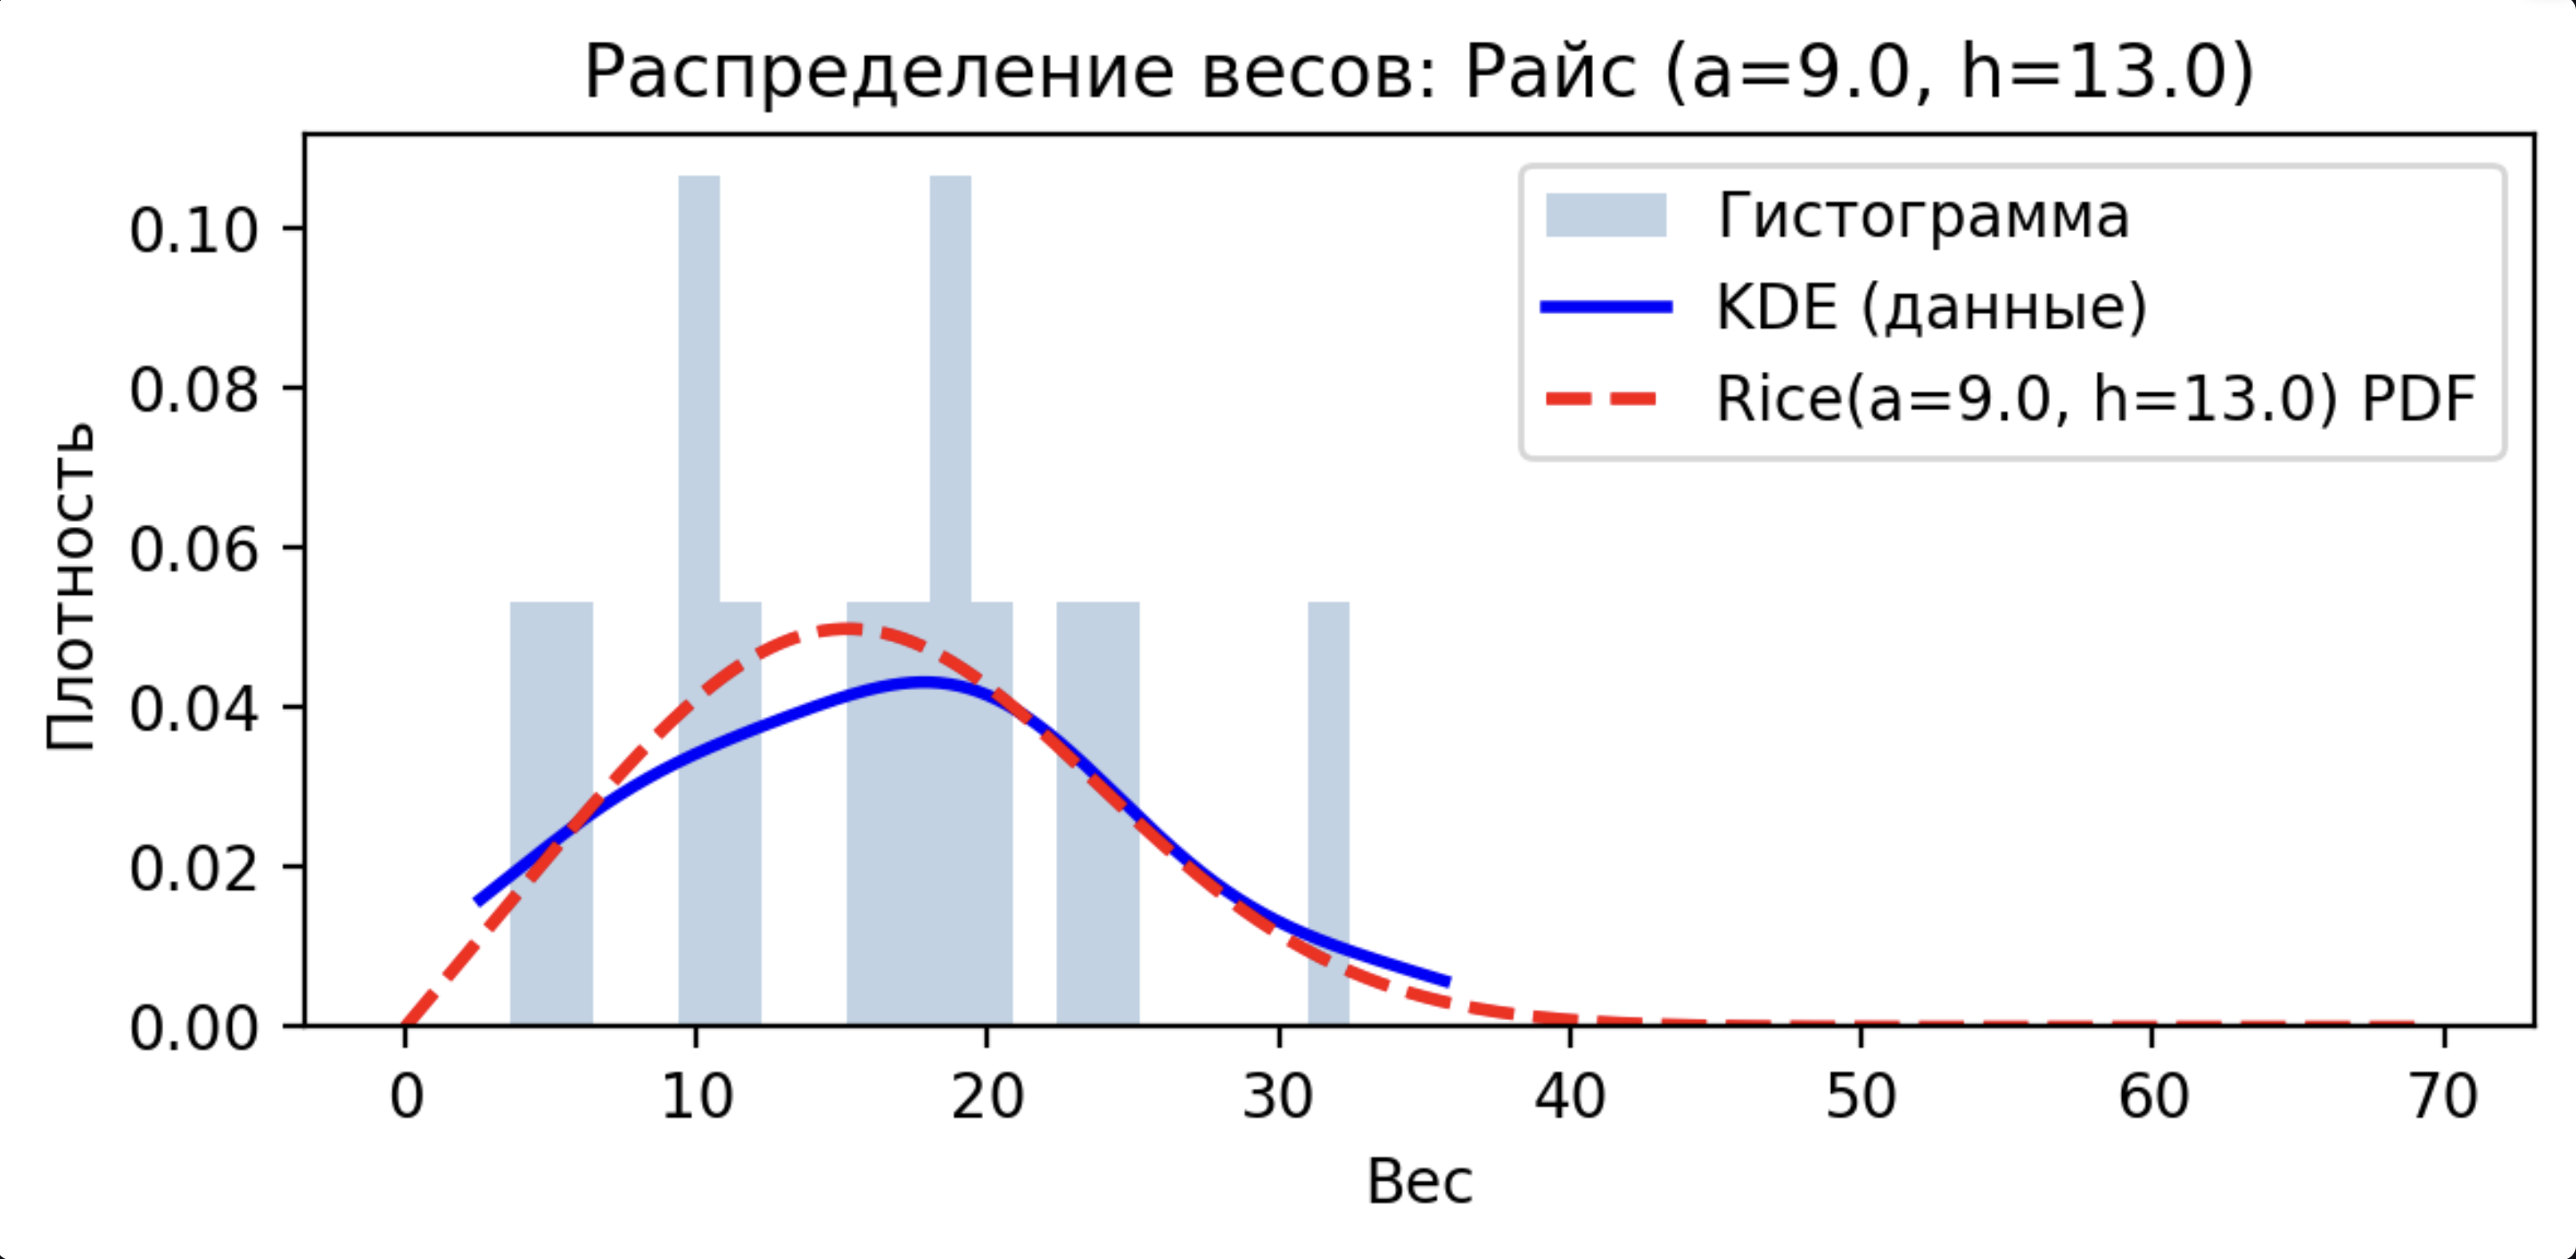
\includegraphics[width=0.7\linewidth]{images/lab1/dist.png}
    \caption{Сгенерированный граф и распределение весов рёбер}
    \label{fig:graph_gen}
\end{figure}

\subsection{Матрицы смежности и весов}

Программа экспортирует две матрицы: матрицу смежности и матрицу
весов. Результат экспорта приведен на рис.~\ref{fig:matrices_adj_weight}.

\begin{figure}[H]
    \centering
    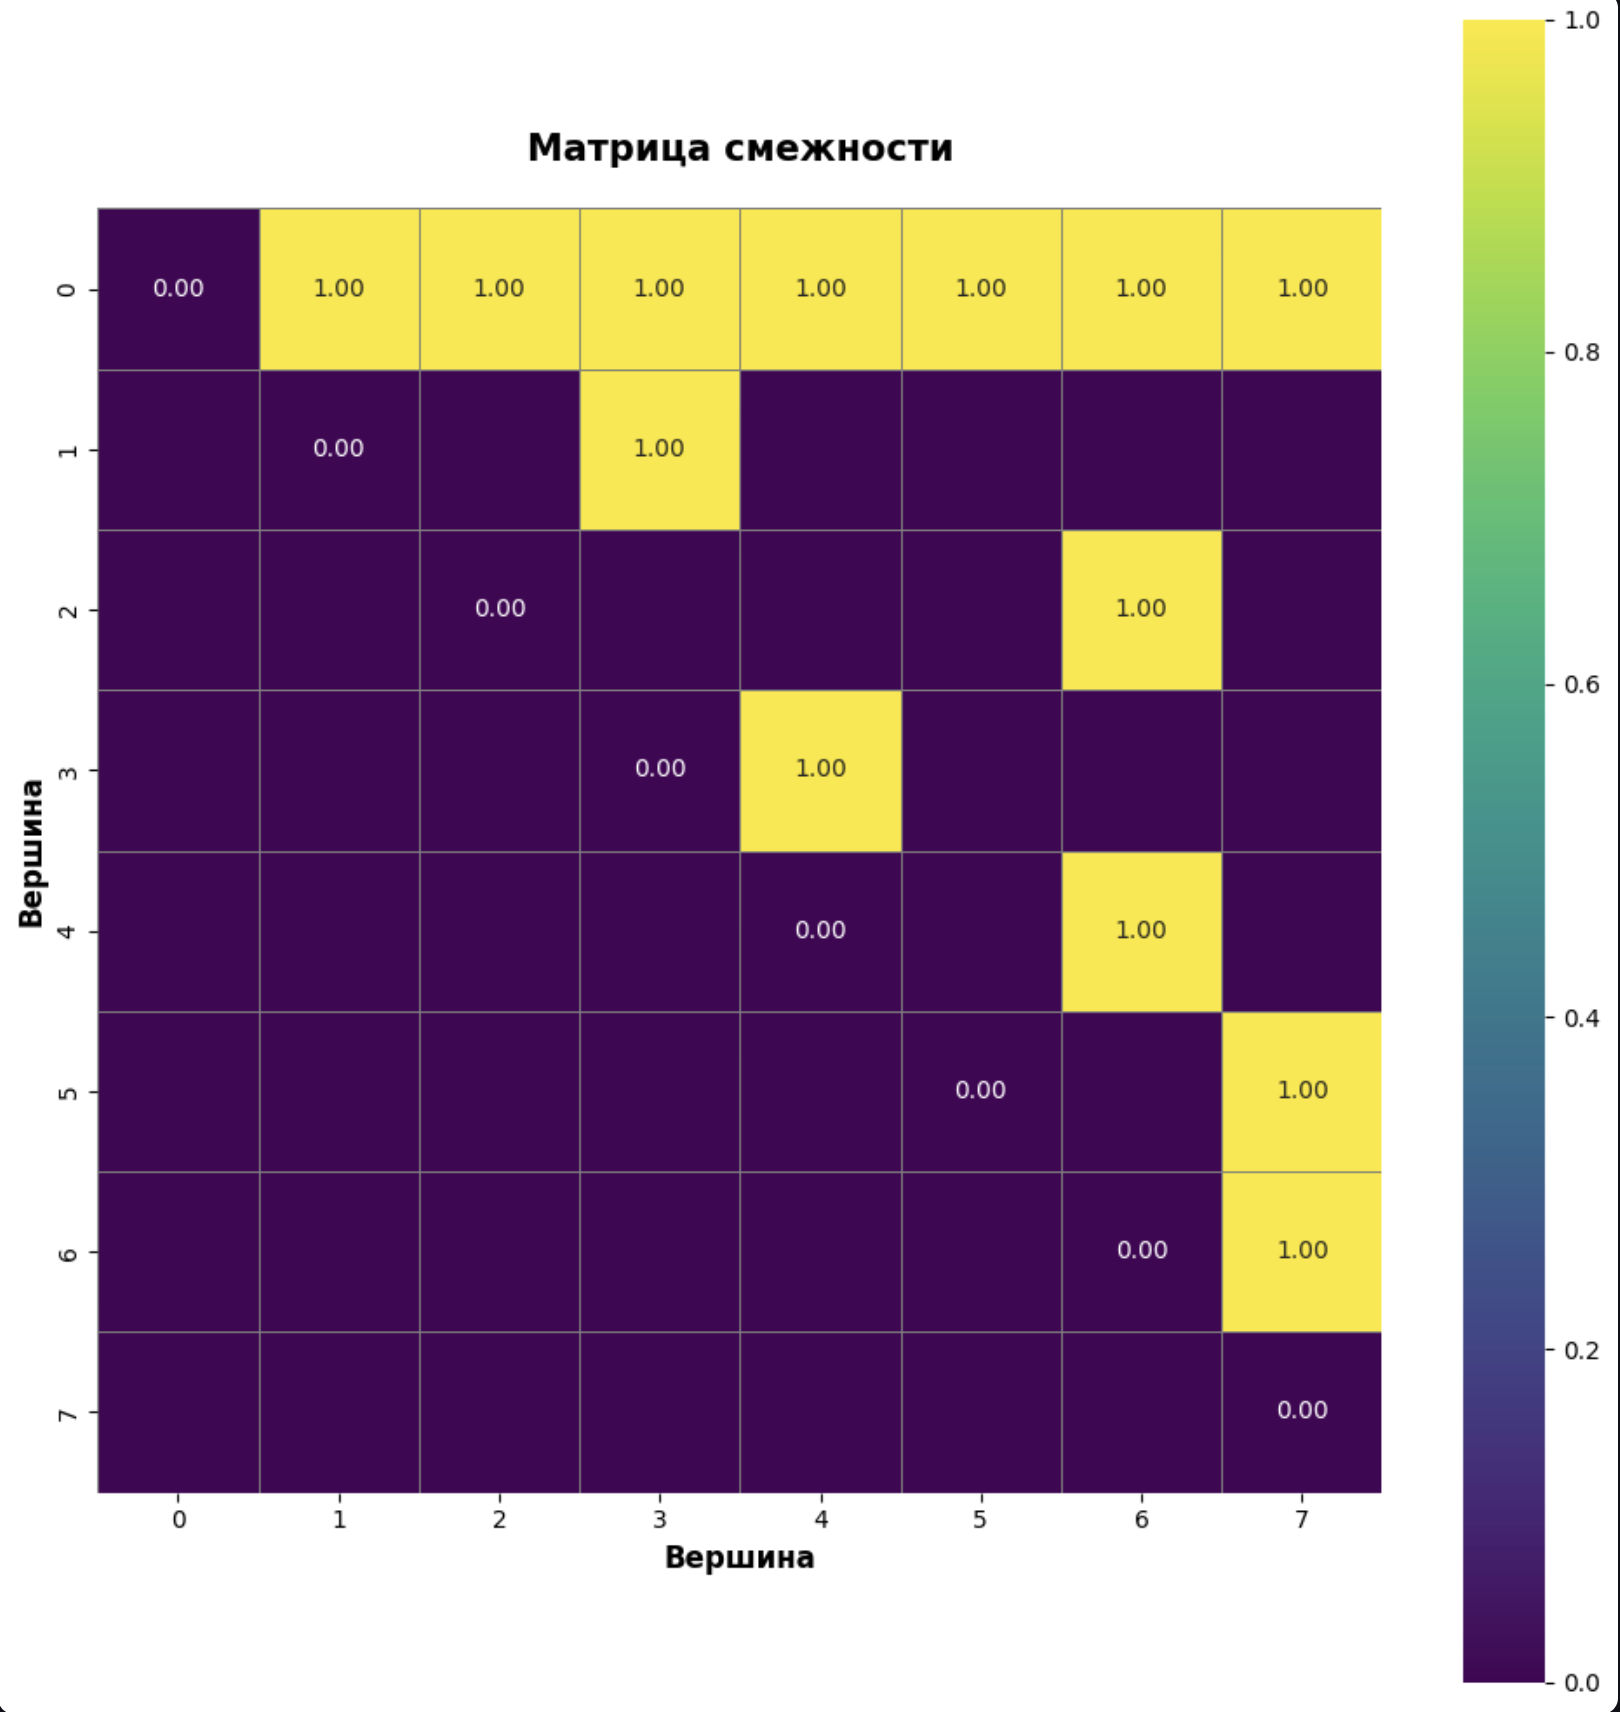
\includegraphics[width=0.48\linewidth]{images/lab1/adjency.png}%
    
\includegraphics[width=0.48\linewidth]{images/lab1/weights.png}
    \caption{Матрица смежности (слева) и матрица весов (справа)}
    \label{fig:matrices_adj_weight}
\end{figure}

\subsection{Метод Шимбелла}

Программа строит и выводит две матрицы: \textit{min} и \textit{max} суммарных весов маршрутов длины ровно $k$. Матрицы для $k=V-1$ показаны на рис.~\ref{fig:shimbell}.

\begin{figure}[H]
    \centering
    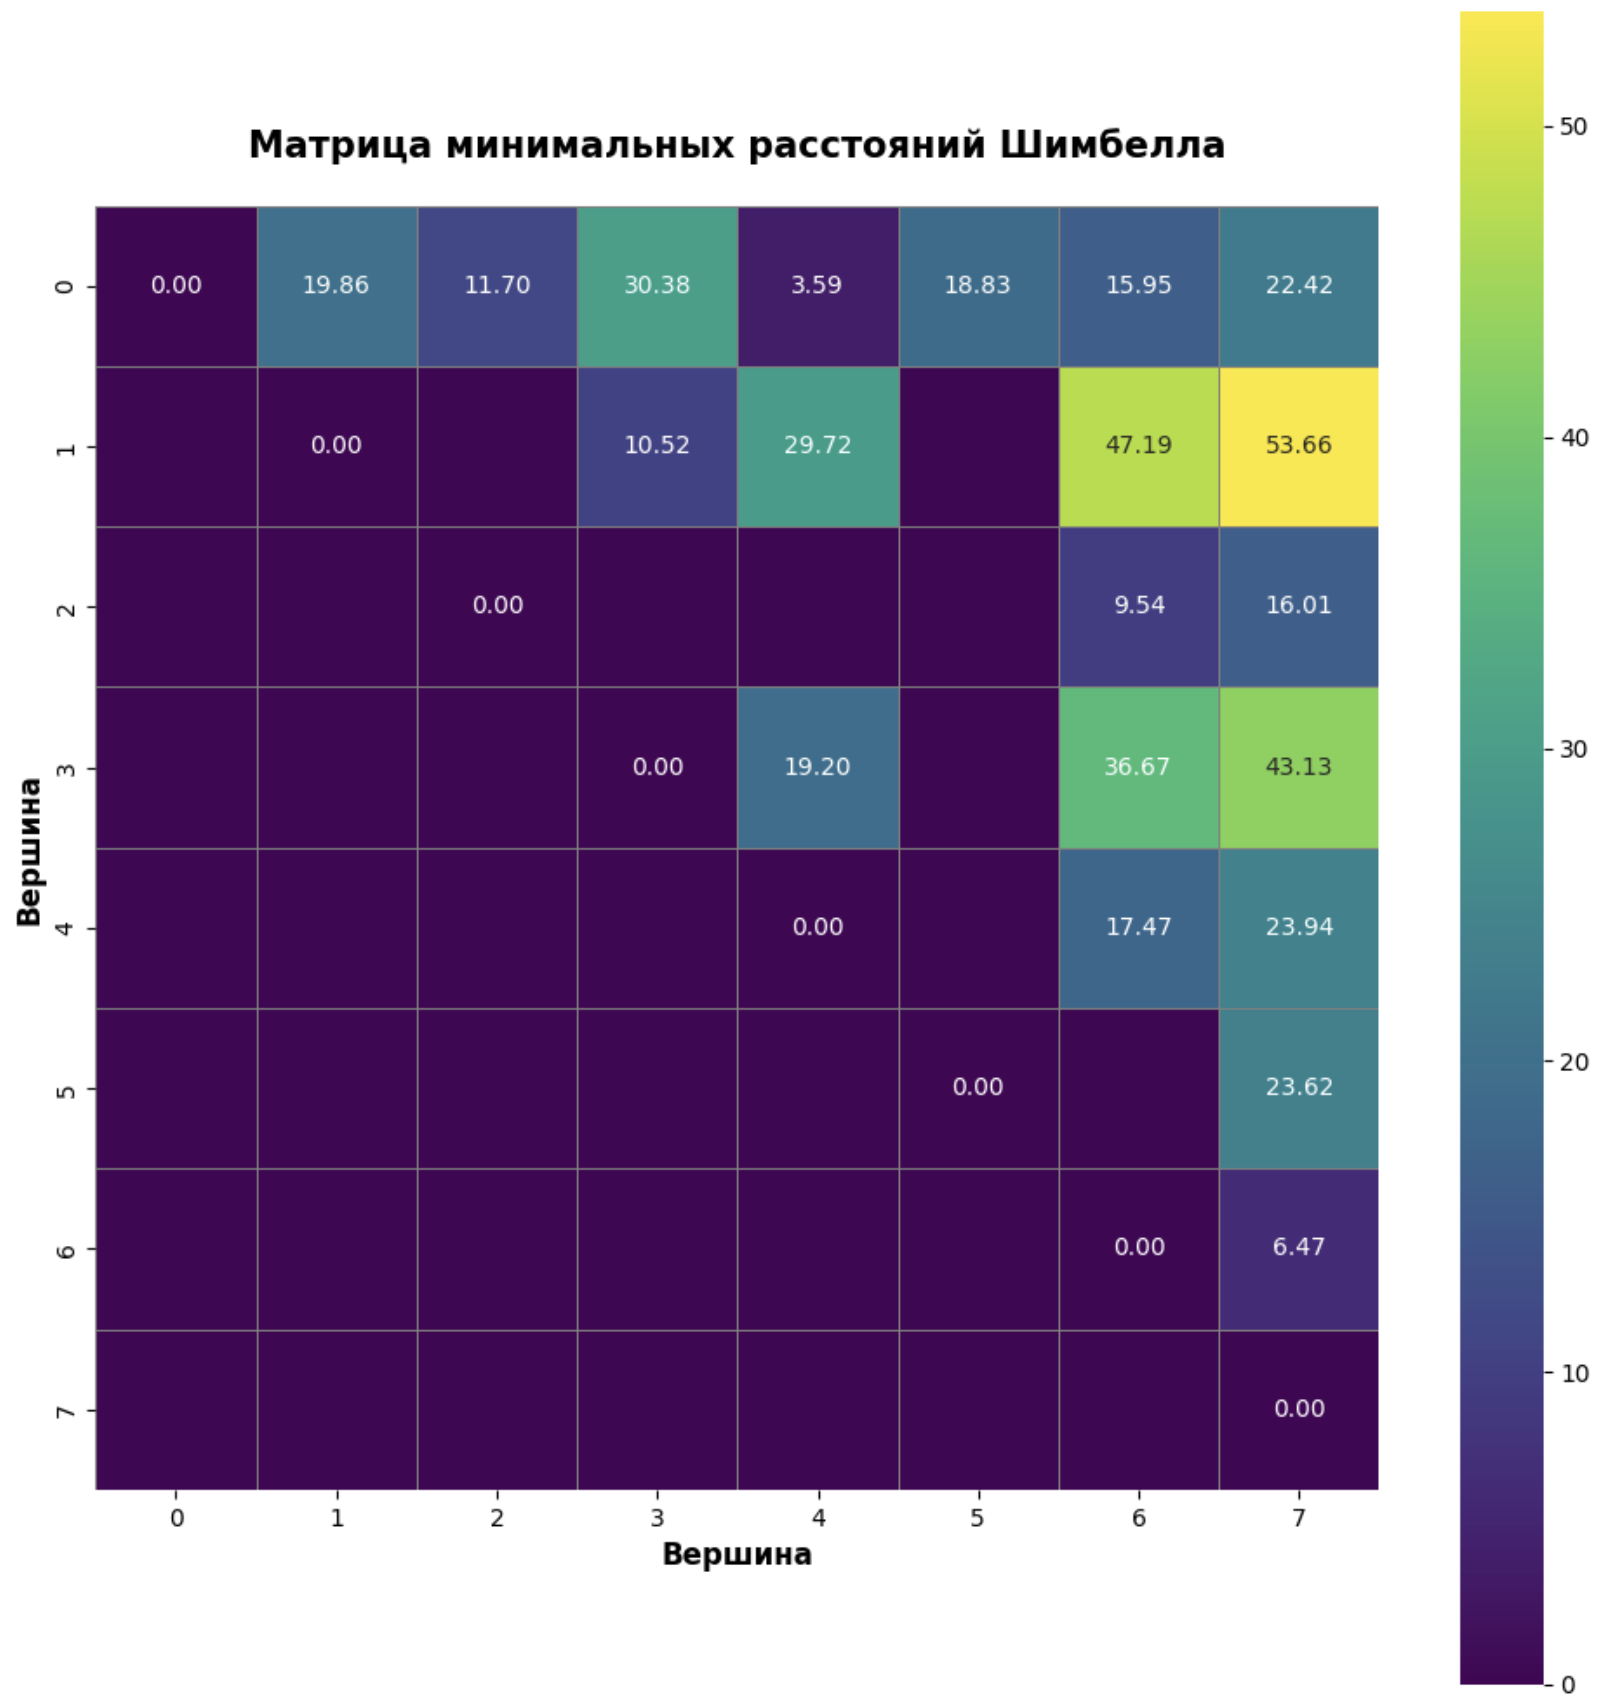
\includegraphics[width=0.48\linewidth]{images/lab1/minshimbell.png}%
    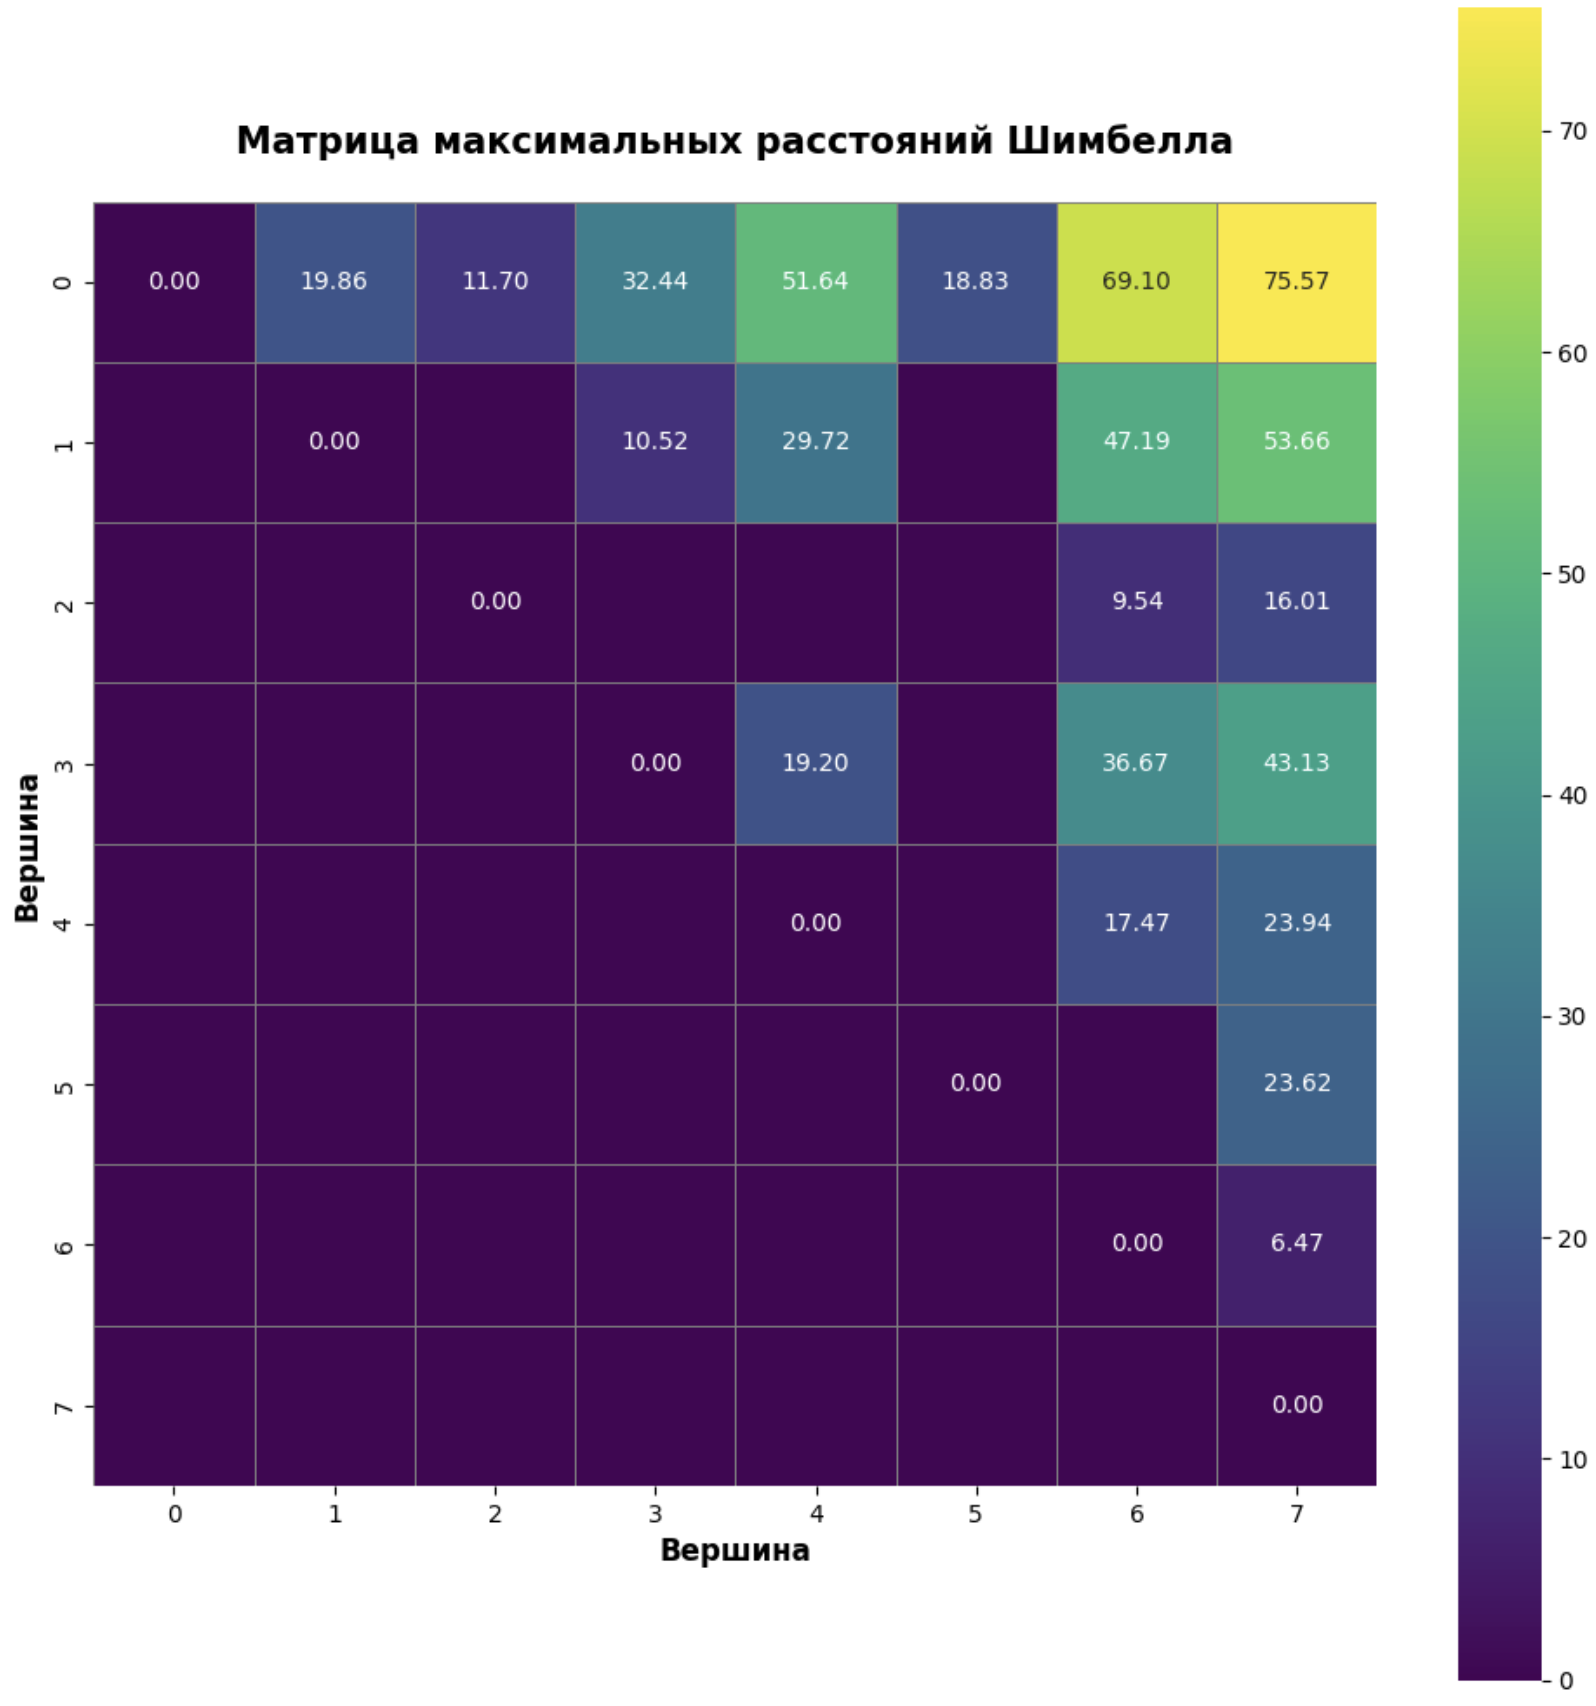
\includegraphics[width=0.48\linewidth]{images/lab1/maxshimbell.png}
    \caption{Матрицы расстояний Шимбелла для $k=V-1$}
    \label{fig:shimbell}
\end{figure}

Все матрицы визуализируются на стороне Python с помощью скрипта \texttt{plot\_matrix.py}, результат отображается в виде тепловой карты. Если значение в исходной матрице отсутствует (\texttt{std::nullopt}), соответствующая ячейка на тепловой карте оставляется пустой. Элементы главной диагонали заменяются нулями для канонического вида.

\subsection{Подсчёт всех маршрутов}

Пользователь вводит вершины-источник и вершину-цель. Программа находит
все простые пути между ними методом поиска с возвратом и выводит их
список в консоль. Визуализация (рис.~\ref{fig:all_paths}) выделяет все найденные пути одновременно: каждый путь~--- своим цветом, рёбра остального графа отображаются серым.

\begin{figure}[H]
    \centering
    
\includegraphics[width=1\linewidth]{images/lab1/paths.png}
    \caption{Все простые маршруты между заданными вершинами}
    \label{fig:all_paths}
\end{figure}

\subsection{Метрики графа: эксцентриситеты, центр, диаметр}

Программа вычисляет эксцентриситет каждой вершины через BFS, находит
радиус, диаметр, центральные и диаметральные вершины. Результаты
выводятся в консоль (рис.~\ref{fig:ecc_text}). На визуализации (рис.~\ref{fig:ecc_graph} и~\ref{fig:ecc_diameter}) вершины раскрашены по роли: центральные~--- одним цветом, диаметральные~--- другим.

\begin{figure}[H]
    \centering
    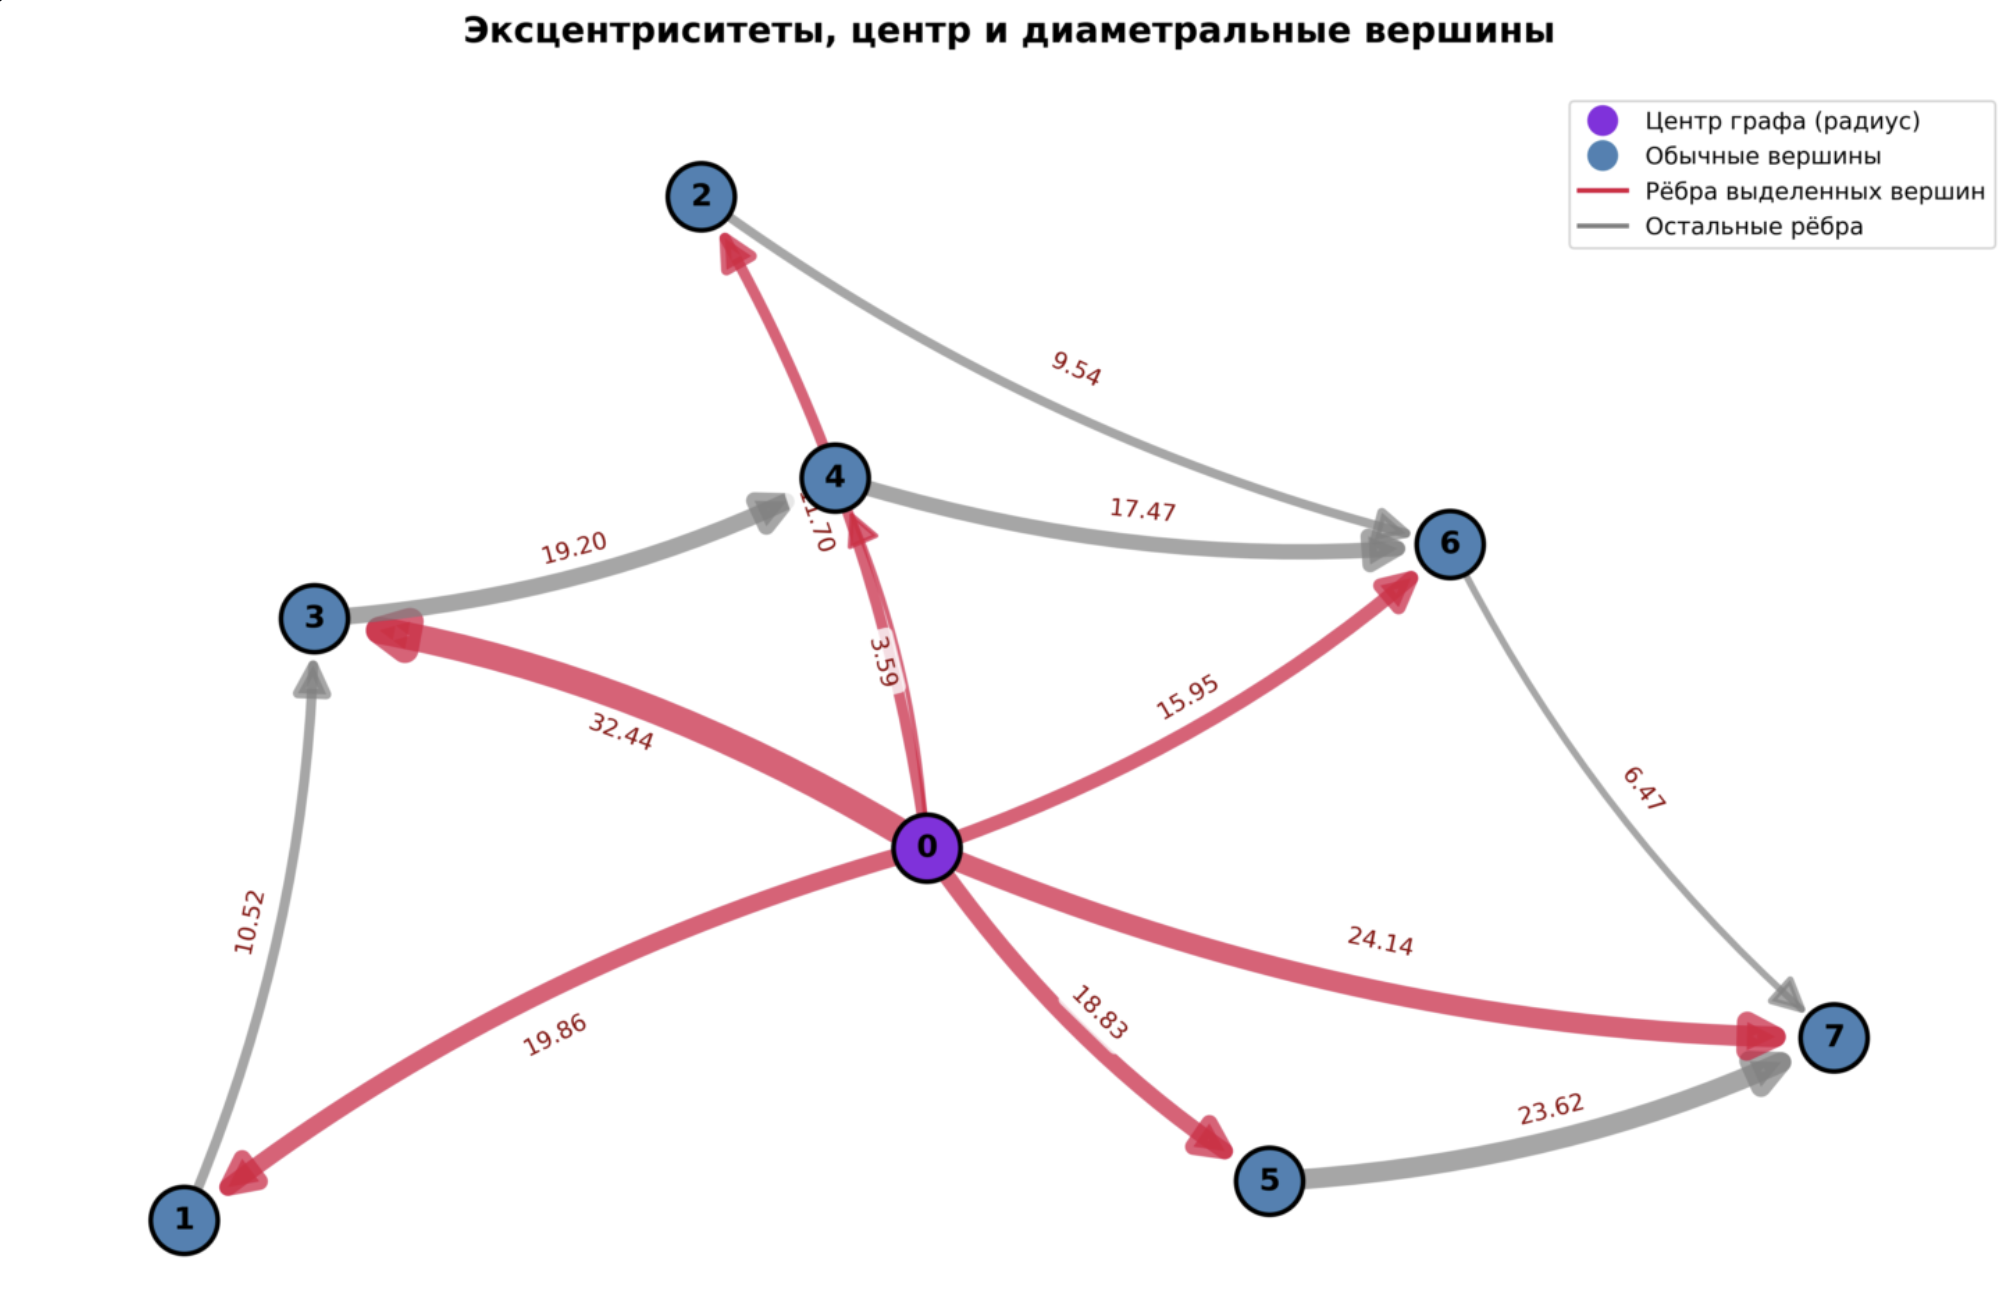
\includegraphics[width=1\linewidth]{images/lab1/exc.png}
    \caption{Орграф с выделением центра}
    \label{fig:ecc_graph}
\end{figure}

\begin{figure}[H]
    \centering
    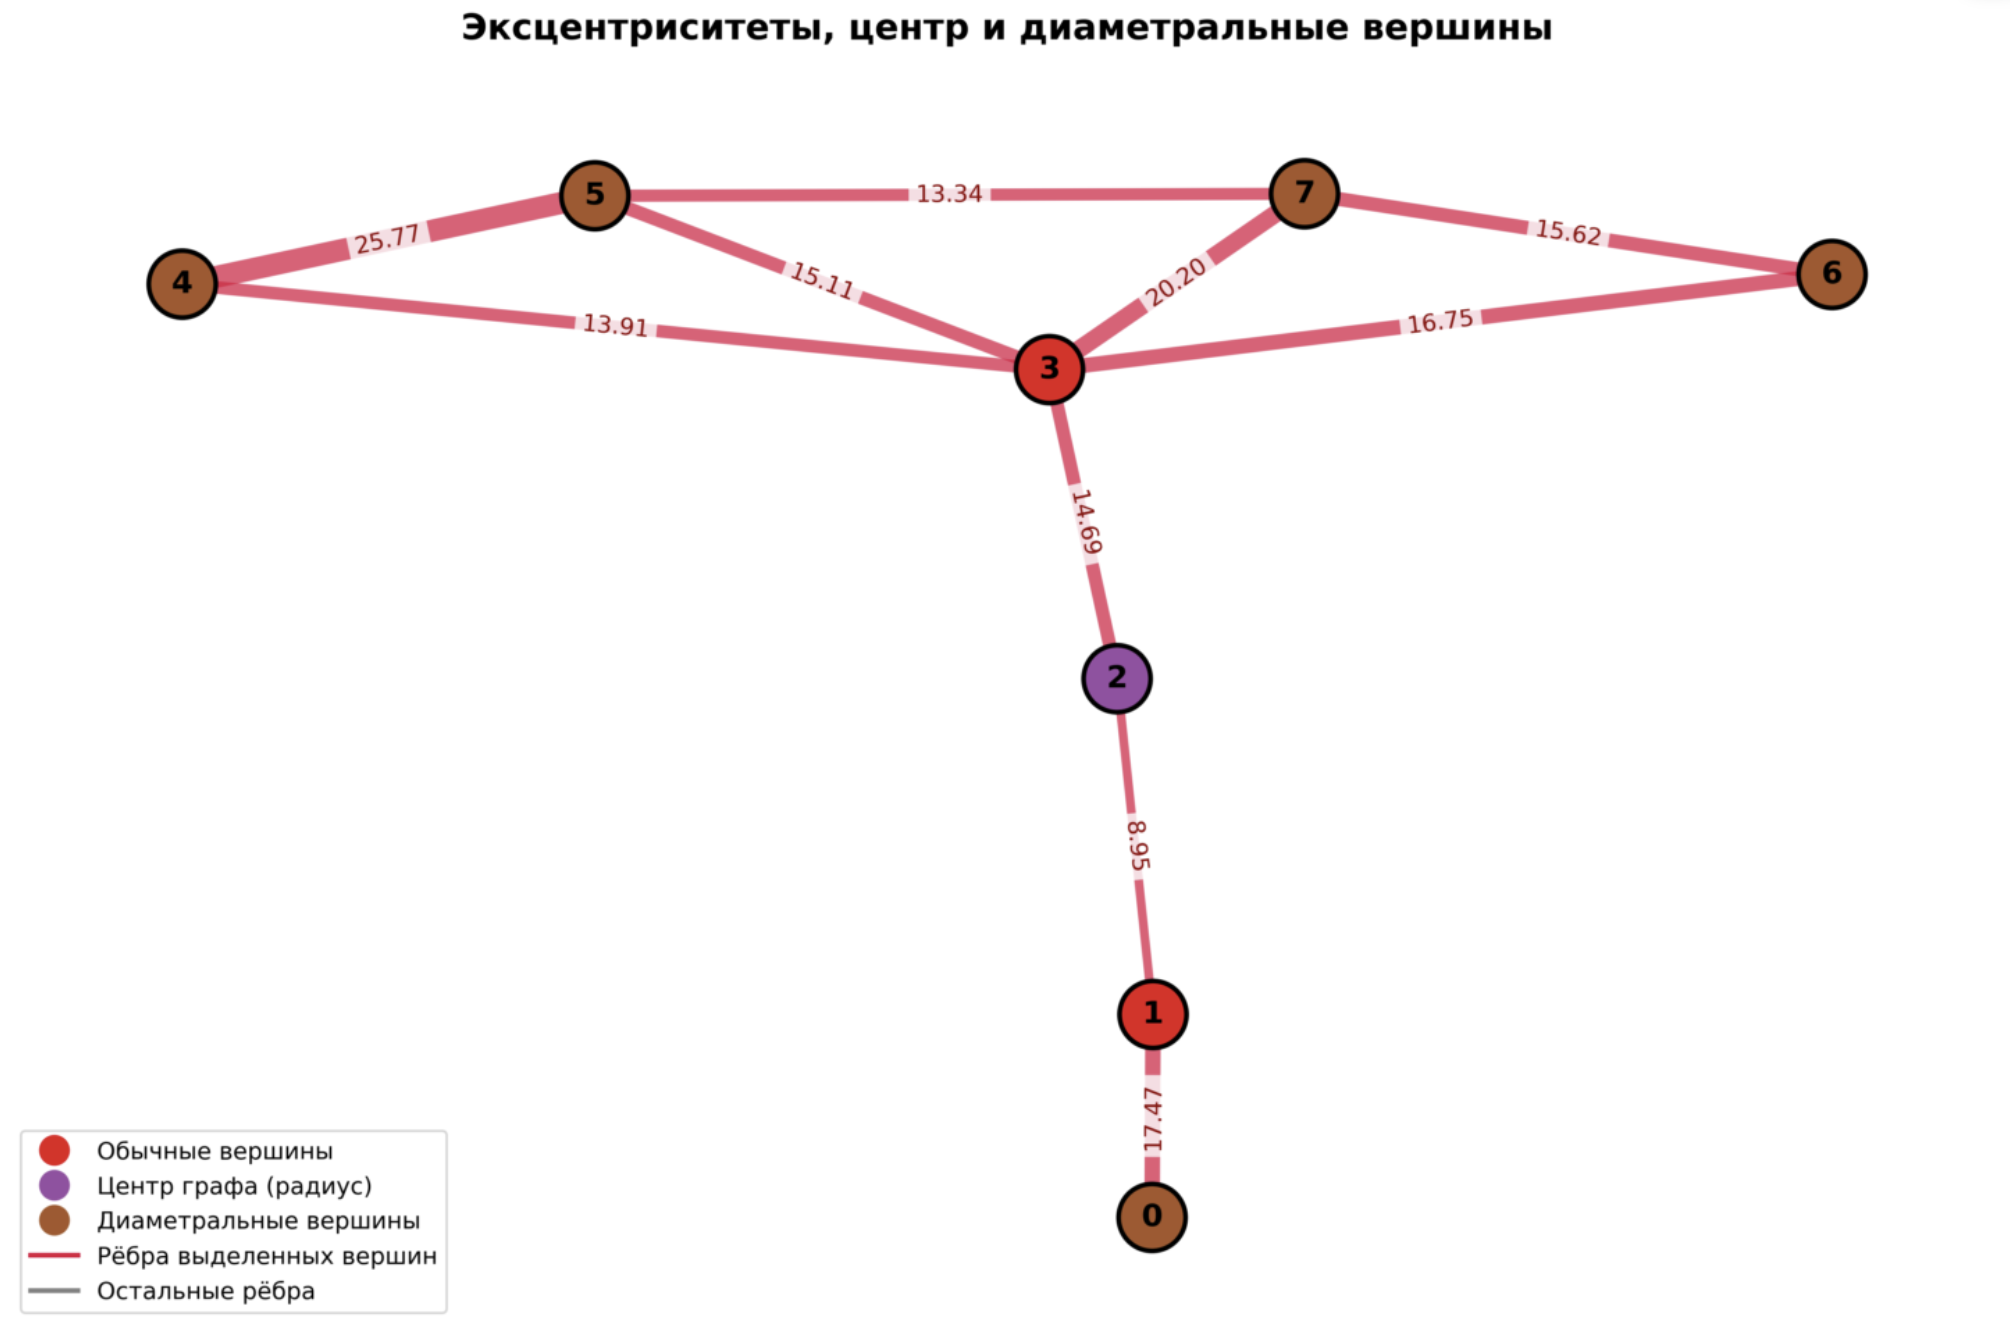
\includegraphics[width=1\linewidth]{images/lab1/exc1.png}
    \caption{Граф с центром и диаметром}
    \label{fig:ecc_diameter}
\end{figure}

\begin{figure}[H]
    \centering
    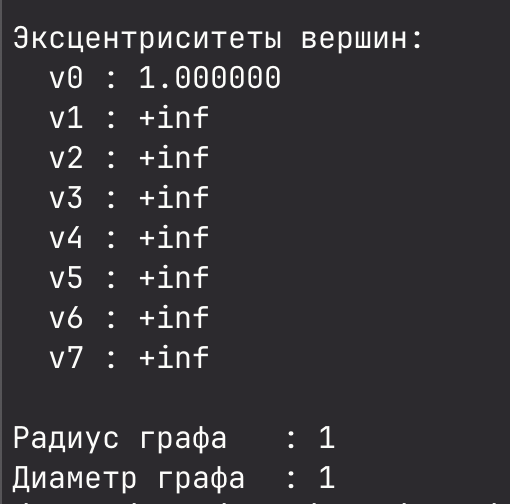
\includegraphics[width=0.4\linewidth]{images/lab1/exctxt.png}
    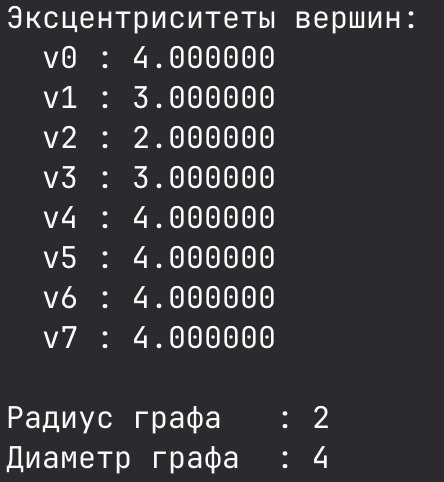
\includegraphics[width=0.362\linewidth]{images/lab1/exctxt1.png}
    \caption{Текстовый вывод метрик графа}
    \label{fig:ecc_text}
\end{figure}

В орграфе ситуация выглядит так: только вершина $v_0$ имеет конечный эксцентриситет, тогда как у всех остальных вершин эксцентриситет равен $+\infty$. В неорграфе эксцентриситеты распределены иначе: минимальное значение равно 2 (вершина $v_2$), максимальное — 4 (вершины $v_0, v_4-v_7$).

\subsubsection{Обход рёбер в ширину}

BFS запускается из вершины, заданной пользователем. Программа выводит
порядок посещения вершин, список рёбер дерева и итоговое число итераций. Рёбра дерева
обхода выделяются на визуализации (рис.~\ref{fig:bfs_tree}).

\begin{figure}[H]
    \centering
    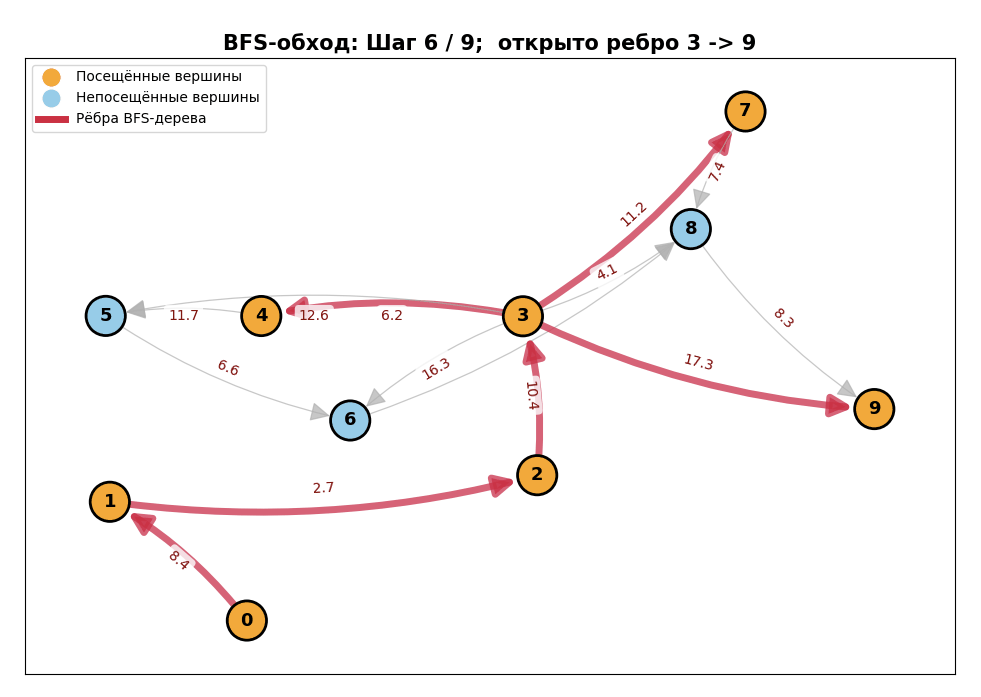
\includegraphics[width=0.82\linewidth]{images/lab2/bfs.png}
    \caption{Граф с выделенными рёбрами дерева BFS-обхода}
    \label{fig:bfs_tree}
\end{figure}

\subsubsection{Алгоритм Дейкстры}

Пользователь вводит начальную и конечную вершины. Программа выводит
вектор расстояний от источника до всех вершин, восстановленный путь
как последовательность вершин и число итераций. Результат поиска кратчайшего пути показан на рис.~\ref{fig:dijkstra}.

\begin{figure}[H]
    \centering
    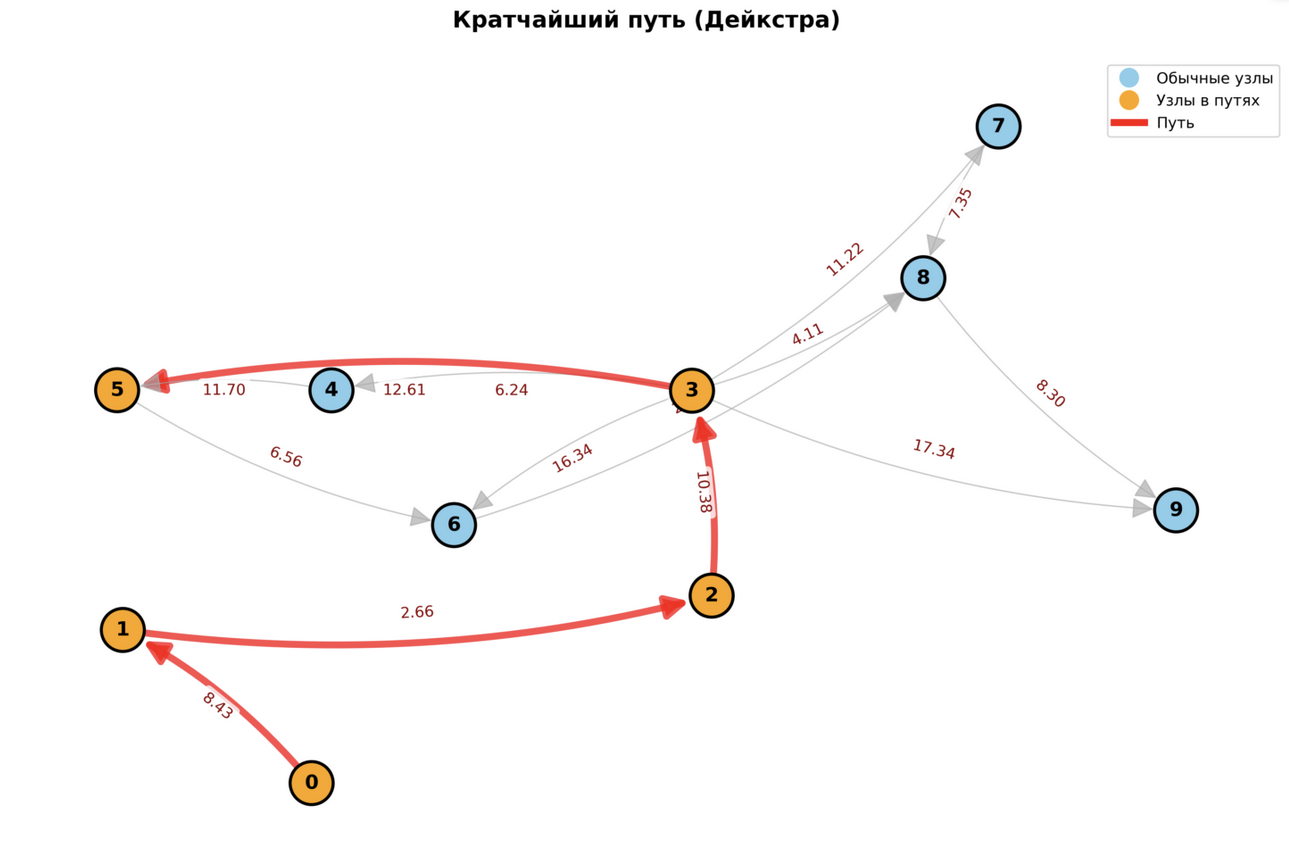
\includegraphics[width=0.9\linewidth]{images/lab2/deijkstra.png}
    \caption{Кратчайший путь по алгоритму Дейкстры}
    \label{fig:dijkstra}
\end{figure}

\subsubsection{Сравнение алгоритмов}

Оба алгоритма запускаются на одном графе с одной стартовой вершиной.
Результат выводится в виде гистограммы (рис.~\ref{fig:compare}): название алгоритма и число итераций. Оба алгоритма считают не только количество обращений к ребрам, но и обращения к внутренним структурам данных. Для теста числа итераций был создан граф с 50 вершинами.

\begin{figure}[H]
    \centering
    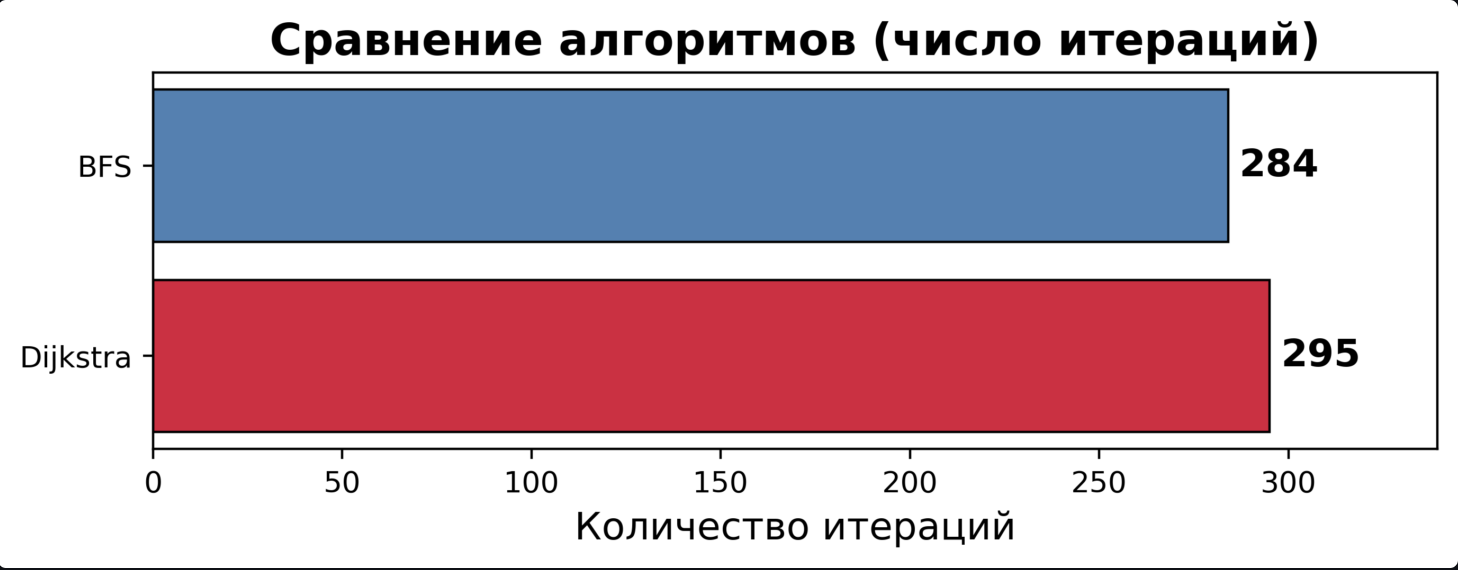
\includegraphics[width=0.7\linewidth]{images/lab2/compare.png}
    \caption{Сравнения числа итераций BFS и Дейкстры}
    \label{fig:compare}
\end{figure}

\subsection{Формирование сети потоков}

На основе ориентированного графа, сгенерированного в предыдущих работах, были сформированы матрицы пропускных способностей $C$ и стоимостей дуг $W$. Значения генерировались случайным образом. Визуализация исходных характеристик сети приведена на рисунках~\ref{fig:flow_network},~\ref{fig:lab3_matrices}.

\begin{figure}[H]
    \centering
    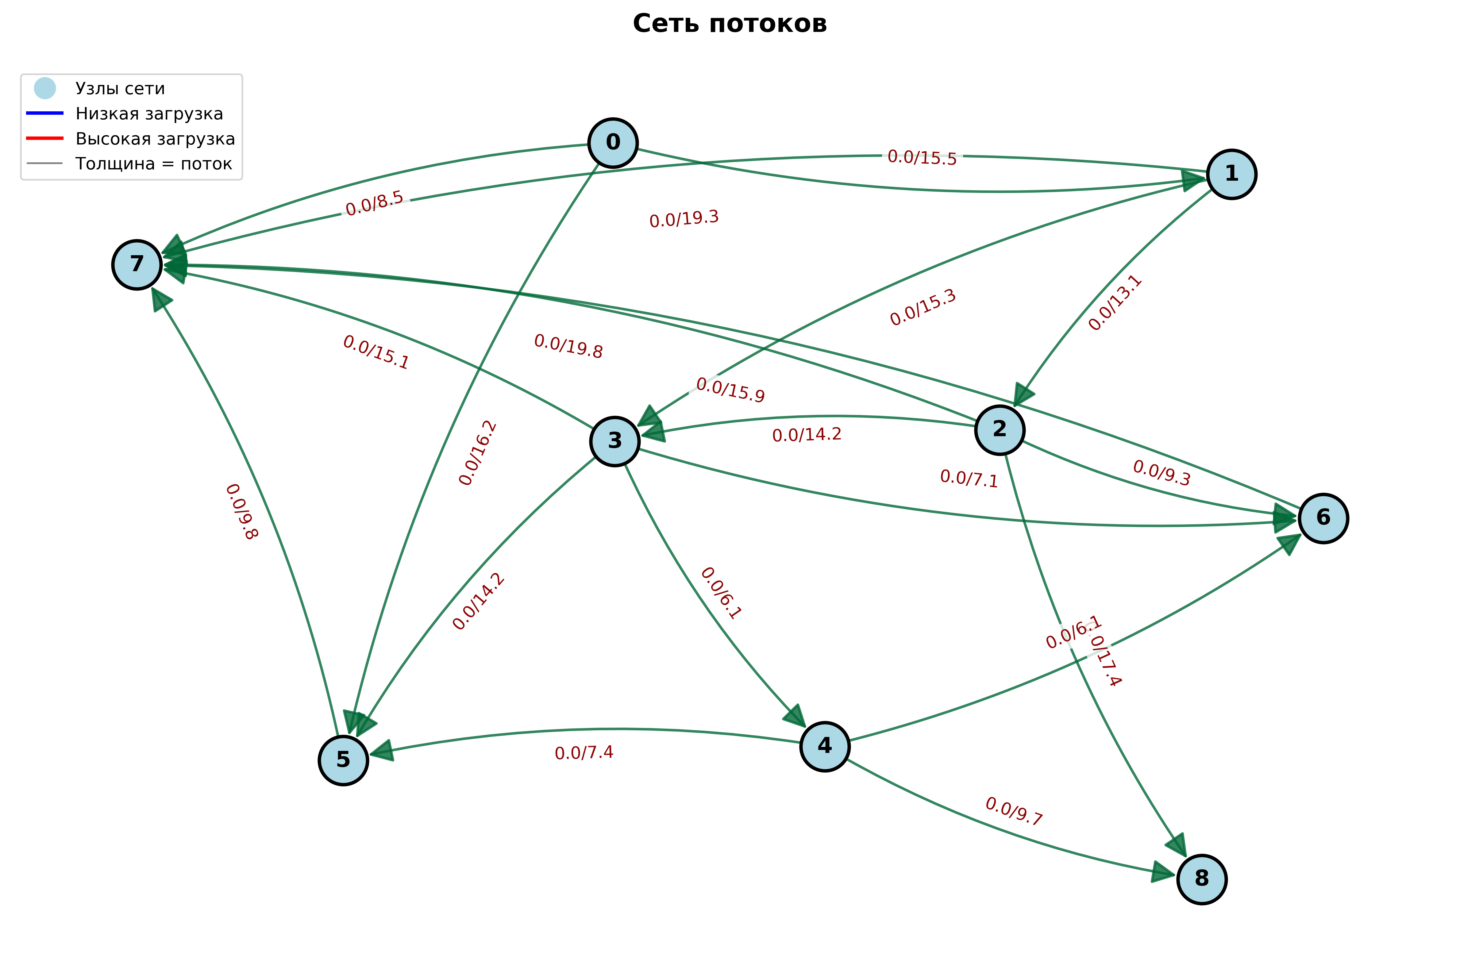
\includegraphics[width=0.82\linewidth]{images/lab3/flow net.png}
    \caption{Сеть потоков}
    \label{fig:flow_network}
\end{figure}

\begin{figure}[H]
    \centering
    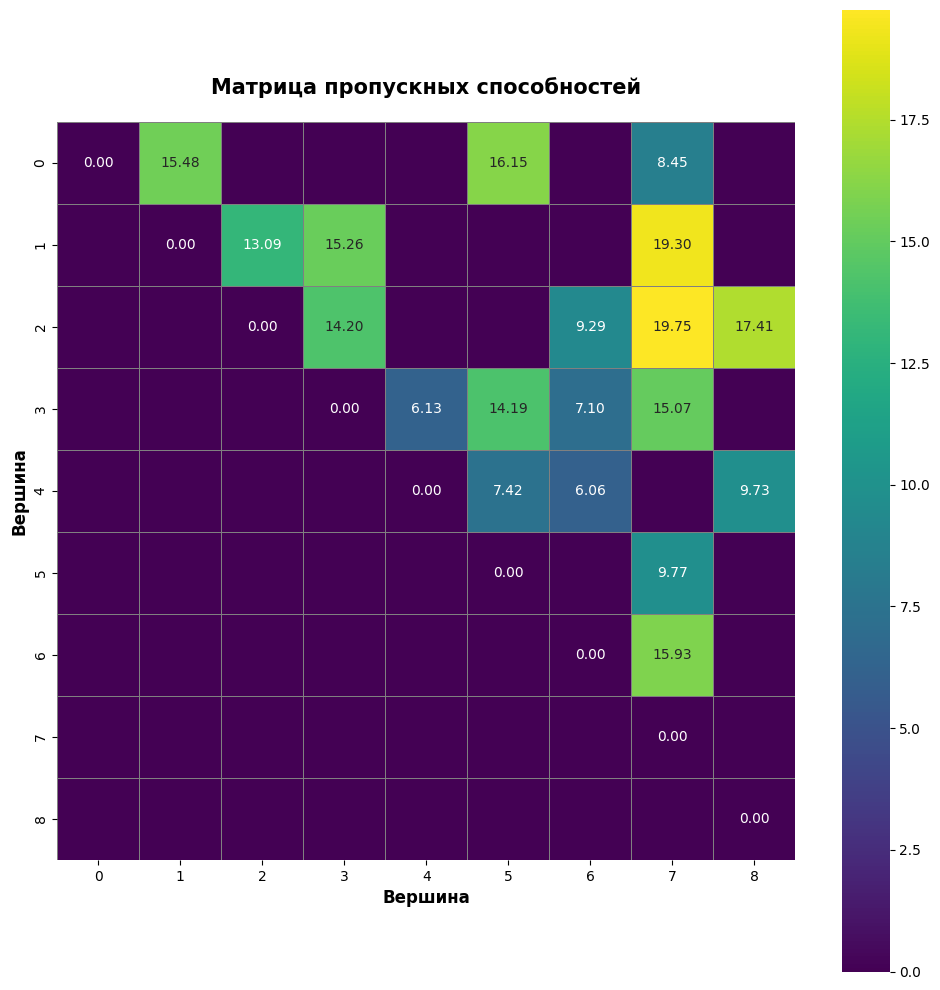
\includegraphics[width=0.48\linewidth]{images/lab3/capacities.png}%
    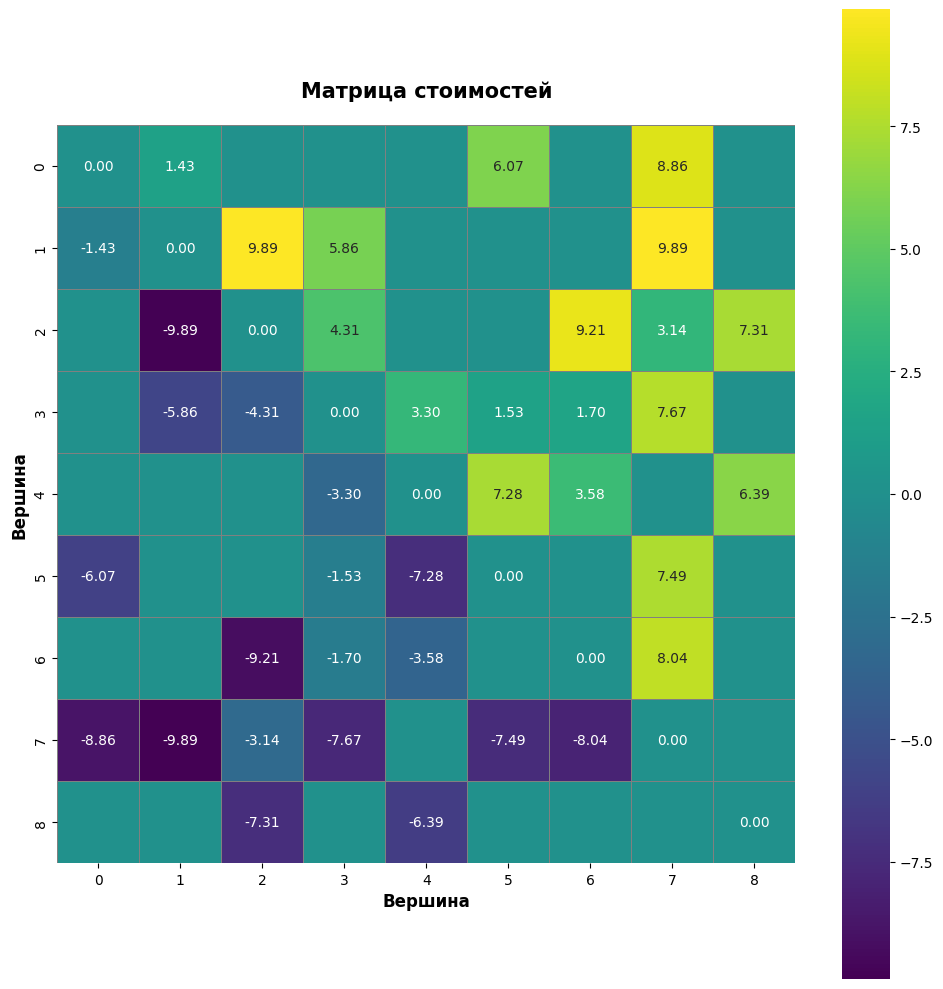
\includegraphics[width=0.48\linewidth]{images/lab3/costs.png}
    \caption{Матрица пропускных способностей матрица стоимостей}
    \label{fig:lab3_matrices}
\end{figure}

\subsection{Алгоритм Форда--Фалкерсона: Максимальный поток}

Для нахождения максимального потока между истоком и стоком использовался алгоритм Форда--Фалкерсона. Программа итеративно находит увеличивающие пути в остаточной сети до тех пор, пока они существуют. 

На рис.~\ref{fig:max_flow_graph} представлена финальная визуализация сети, из 1 в 7 вершину.

\begin{figure}[H]
    \centering
    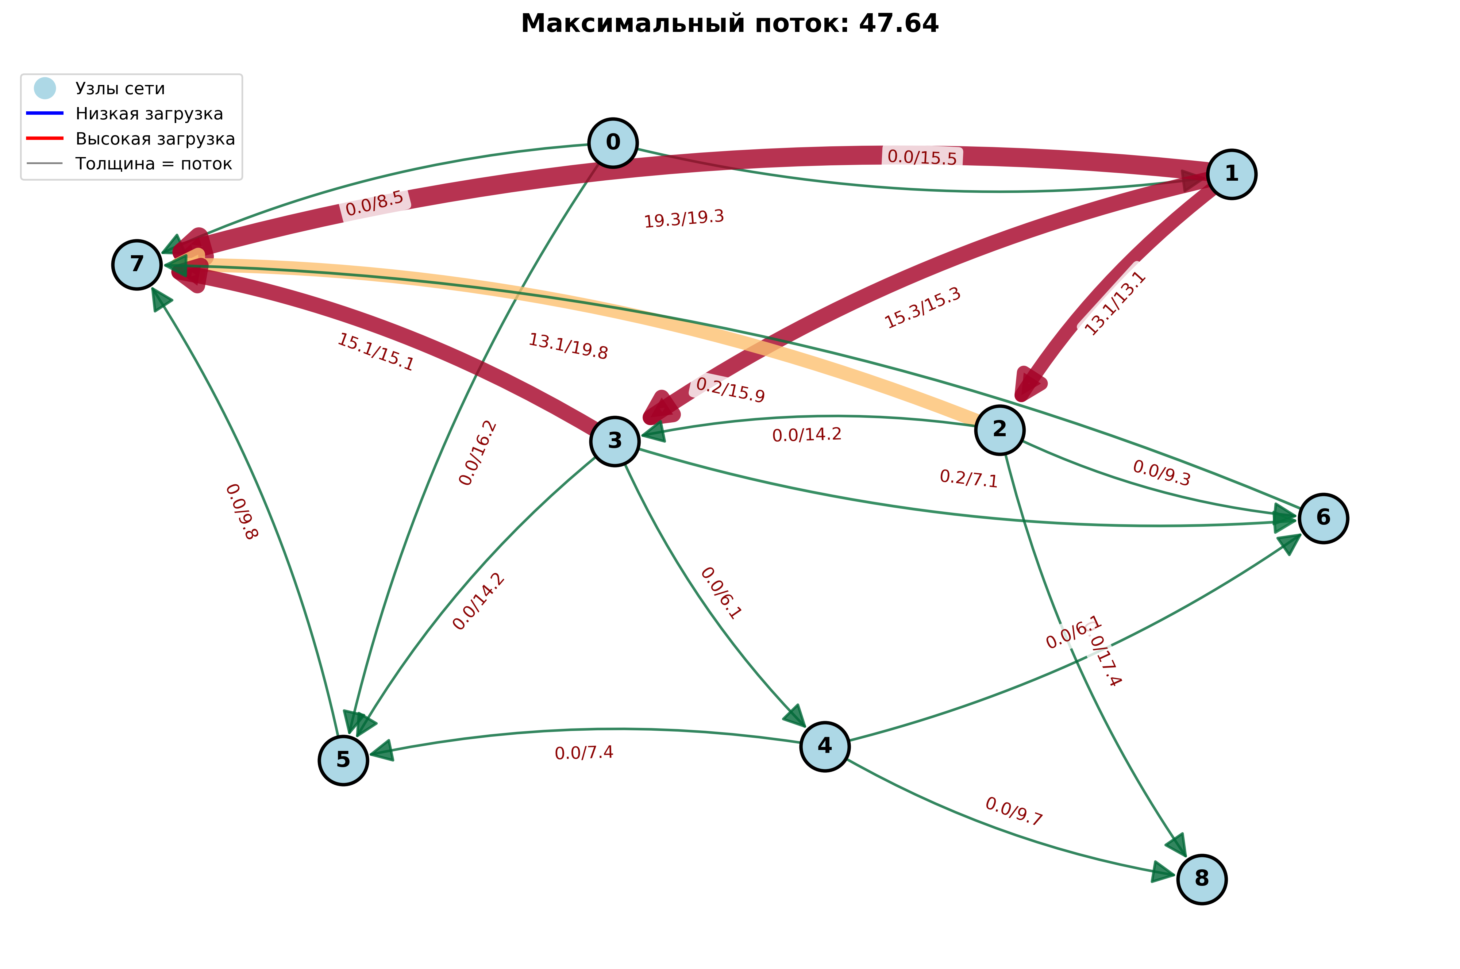
\includegraphics[width=0.8\linewidth]{images/lab3/max_flow.png}
    \caption{Распределение максимального потока в транспортной сети}
    \label{fig:max_flow_graph}
\end{figure}

\subsection{Поток минимальной стоимости}

Согласно заданию, был выполнен расчет потока заданной величины $F = \lfloor \frac{2}{3} \cdot F_{max} \rfloor$. Для минимизации суммарной стоимости использовался алгоритм поиска кратчайших путей в остаточной сети (на базе алгоритма Беллмана--Форда, позволяющего корректно обрабатывать веса дуг).

Результаты распределения потока и итоговая суммарная стоимость представлены на рис.~\ref{fig:min_cost_res}.

\begin{figure}[H]
    \centering
    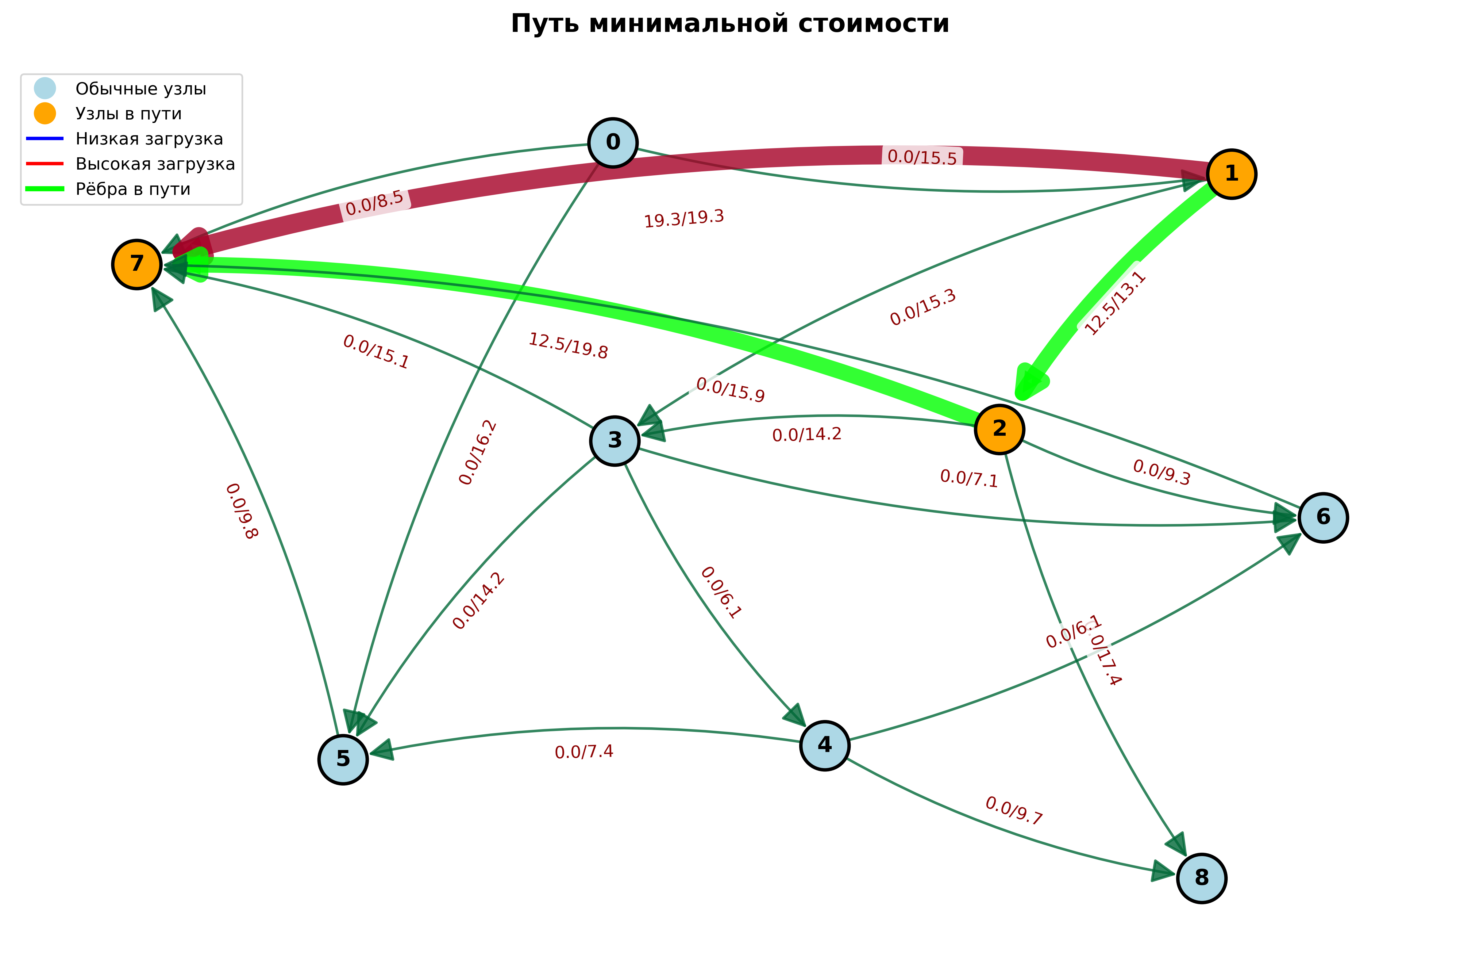
\includegraphics[width=0.8\linewidth]{images/lab3/min_cost.png}
    \caption{Визуализация потока минимальной стоимости для величины $2/3$ от максимального}
    \label{fig:min_cost_res}
\end{figure}

\begin{figure}[H]
    \centering
    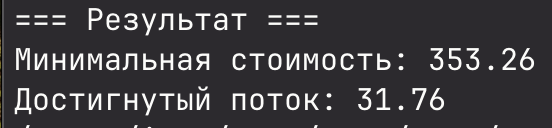
\includegraphics[width=0.5\linewidth]{images/lab3/min_cost_output.png}
    \caption{Консольный вывод: значение потока, итоговая стоимость и количество итераций}
    \label{fig:min_cost_console}
\end{figure}

Программа успешно нашла оптимальное распределение. Как видно из рис.~\ref{fig:min_cost_console}, алгоритм прекратил работу ровно при достижении заданного пользователем значения потока, выбрав пути с наименьшей суммарной стоимостью дуг.